\chapter{Generative Taggers using Finite-State Machines}
\label{chap:fsm}
In this Chapter, I will present an implementation of HMMs using {\it
  weighted finite-state machines}. It is further investigated in
Publications \ref{pub:1} and \ref{pub:2}. The implementation allows
for extensions of the HMM model in the spirit of \cite{Halacsy2007},
who utilize label context in the emission model of an HMM. It also
allows for applying global grammatical constraints. I will first
present a short summary of the most important aspects of finite-state
calculus and then present the finite-state implementation of HMMs.

\section{Weighted Finite-State Machines}

\paragraph{Automata} Weighted Finite-state automata are a data
structure for representing algorithms that solve the decision problem
of a regular language. A string can be either accepted or discarded
by a an automaton with some weight. Typically, weights bear
resemblance to probabilities and if they are interpreted as
probabilities, an automaton defines a distribution over the set of
strings. 

Figure \ref{fig:np-fsm} presents a finite-state which recognizes a
subset of noun phrases in the Penn Treebank. It illustrates the key
components of a finite-state automaton $M$
\begin{enumerate}
\item A finite set of states $Q_M$ ($\{0,\ 1,\ 2,\ 3,\ 4\}$ in Figure \ref{fig:np-fsm}).
\item An alphabet $\Sigma_M$ (the POS labels in Penn Treebank in Figure \ref{fig:np-fsm}).
\item A unique initial state $I_M$ ($0$ in Figure \ref{fig:np-fsm}).\footnote{Some formulations allow for several initial states with initial weights. This does, however, not increase the expressiveness of the formalism.}
\item A set of final states $F_M = \{r_1, ..., r_m\} \subset Q_M$ with associated final weights ${\rm f}(r_i)$ ($\{2\}$ and $1.0$ in Figure \ref{fig:np-fsm}).\footnote{Alternatively, we could also specify a final weight for every state. Then the actual final states would be the ones wit non-zero weight.}
\item A transition function $\tau_M$, which specifies a, possibly empty, set 
$$\tau_M(q,x) = \{(q_1,w_1),\ ...,\ (q_n,w_n)\}$$ of target states and transition weights for each symbol $x\in \Sigma_M$ in each state $q \in Q_M$ (in Figure, \ref{fig:np-fsm} the relation is represented by the arrows in the graph).
\end{enumerate}
\begin{figure}[!ftb]
\begin{center}
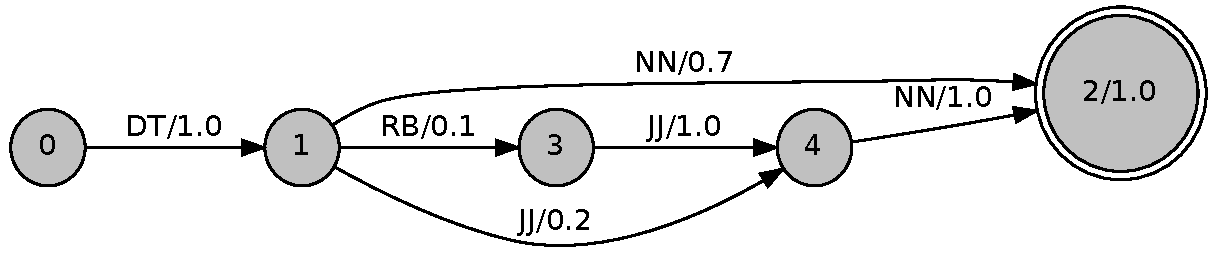
\includegraphics[scale=.65]{np}
\end{center}
\caption{A finite-state machine accepting a subset of the singular noun phrases in Penn Treebank.}\label{fig:np-fsm}
\end{figure}
When $\tau_M(a,q)$ is either empty or a singleton set for all $a$ and $q$, the automaton $M$ is called {\it deterministic} and I write $\tau_M(a,q) = (q_1,w_1)$ instead of $\tau_M(a,q) = \{(q_1,w_1)\}$.

\paragraph{Weight Semirings} Transition and final weights should form a
algebraical structure $\mathbb{K}$ called a semiring which is an abstraction of the
structure of positive real numbers under addition and multiplication. Consequently, two operations, addition $\oplus$ and
multiplication $\otimes$, are defined in $\mathbb{K}$. The addition operation should be
associative, commutative and have an identity element
$\mathbb{0}$. The multiplication operation should also be associative
and commutative. If it has an identity element, that element is
denoted by $\mathbb{1}$. Multiplication should distribute over
addition \citep{Allauzen2007}.

As noted above, the prototypical example of a weight semiring is given by the positive real numbers with the regular addition and multiplication of reals. This weight semiring, called the {\it probability semiring},\footnote{Even though the probability semiring is intended for representing probability distributions, weights cannot be restricted to $[0,1]$ because the semiring has to be closed under addition.}  can be used to represent a probability distribution over the set of strings. In practice, this weight semiring is however rarely used. Because of numerical stability concerns, a logarithmic transformation $x \mapsto -log(x)$ is often applied to the weights and operations in the probability semiring. This gives the {\it log semiring}, where weights belong to $\mathbb{R}$, multiplication is given by $x \otimes y = x + y$ and addition by $x \oplus y = -\log(\exp(-x) + \exp(-y))$.

The addition operation of the log semiring $-\log(\exp(-x) + \exp(-y))$
is slow in practice. Moreover, $-\log(\exp(-x) + \exp(-y)) \approx x$
when $x \ll y$. Therefore, the addition operation in the log semiring
is often replaced by $x \oplus y = \min(x,y)$. This gives the {\it
  tropical semiring} which is the semiring used in this thesis.

I denote the transition weight of the transition leaving state $q_1$
with symbol $x$ and ending up in $q_2$ by $\w(\tau_M(q_1,x), q_2)$. As
a notational convenience, $\w(\tau_M(q_1,x), q_2) = \mathbb{0}$, if
there is no transition from $q_1$ to $q_2$. An automaton $M$ assigns a
weight to a path of states $p = (q_0,\ ...,\ q_{n+1})$, where $q_0 =
I_M$ and $q_n \in F_M$, and a string $s = s_1...s_n \in
\Sigma_M^{n}$. The weight is $\w_M(s,p)$ is given by Equation
\ref{eq:path-weight}. The total weight $\w_M(s)$ assigned to string
$s$ by automaton $M$ is given by Equation \ref{eq:string-weight}
\begin{equation}
\w_M(s,p) =
{\rm f}(q_{n+1})\otimes \bigotimes_{i = 0}^n \w_M(\tau_M(q_i,s_i), q_{i+1})\label{eq:path-weight}
\end{equation}

\begin{equation}
\w_M(s) =
\bigoplus_{p \in Q_M^{n+1}} \w_M(s,p) \label{eq:string-weight}
\end{equation}

\paragraph{Closure Properties} It is well known that regular languages
are closed under many unary and binary operations: union, negation,
concatenation and reversion \citep{Sipser1996}. Similarly, the class
of weighted finite-state machines is closed under these operations and
efficient algorithms for computing these operations exist. Table
\ref{tab:fs-algebra}, summarizes the properties of these algorithms.

\paragraph{Optimization} As stated above, a finite state machine where
each symbol and state is associated to maximally one transition is
called deterministic. It is well known that every finite-state machine
corresponds to a deterministic machine and this holds for weighted
finite-state machines as well given light assumptions on the weight
semiring \citep{Mohri2002}. A determinization algorithm can be applied
to any weighted finite-state machine in order to produce a
deterministic machine which accepts exactly the same set of weighted
strings as the original machine.

\paragraph{N-Best} The finite-state implementation of morphological
taggers presented in Publications \ref{pub:1} and \ref{pub:2} compiles
a weighted finite-state machine which represents a sentence and all of
its alternative label sequences as paths. The path weights correspond
to the joint probabilities of the sentence and label sequences. An
n-best algorithm \citep{Mohri2002} can then be used to efficiently
extract the path that carries the highest probability. The best path
can be found in time $O(|Q| \log(|Q|) + |\tau|)$, where $Q$ is the state
set of the sentence machine and $|\tau|$ is the number of transitions
in the machine.

\begin{table}[!ftb]
\begin{center}
\begin{tabular}{l|l|l}
\hline
Operation & Symbol & Definition \\
\hline
{Power} & {$M^n$} & $\w_{M^n}(s) = \bigoplus_{s_1 ... s_n = s} \w_{M}(s_1) \otimes ... \otimes \w_{M}(s_n)$\\ 
Closure & $\bigoplus_{n = 0}^\infty M^n$ &  \\
Union & $M_1 \oplus M_2$ & $\w_{M_1 \oplus M_2}(s) = \w_{M_1}(s) \oplus \w_{M_2}(s)$\\ 
Concatenation & $M_1.M_2$ & $\w_{M_1.M_2}(s) = \bigoplus_{s_1s_2 = s} \w_{M_1}(s_1) \otimes \w_{M_2}(s_2)$\\
Intersection & $M_1 \cap M_2$ & $\w_{M_1 \cap M_2}(s) = \w_{M_1}(s) \otimes \w_{M_2}(s)$ \\
Composition & $M_1 \circ M_2$ & $\w_{M_1 \circ M_2}(s{\rm :}t) = \bigoplus_{r} \w_{M_1}(s{\rm :}r) \otimes \w_{M_2}(r{\rm :}t)$\\
\end{tabular}
\caption{A selection of operators for weighted finite-state machines
  given by
  \cite{Allauzen2007}.}\label{tab:fs-algebra}
\end{center}
\end{table}

\section{Finite-State Implementation of Hidden Markov Models} As seen
in Chapter \ref{chapter:hmm}, a generative HMM can be decomposed into
an emission model $p(x_i|y_i)$ of emissions $x_i$ given states $y_i$ a
transition model $p(y_{n+1} | y_1, ..., y_n)$, which models the
conditional distribution of a state $y_{n+1}$ given a state history
$y_1, ..., y_n$. As shown in Publications \ref{pub:1} and \ref{pub:2}
both of these can be compiled into weighted finite-state machines.

A generative HMM can be represented as a weighted finite-state machine
in several ways. The implementation presented in Publication
\ref{pub:1}, however, allows for enriching the emission model by
conditioning them on neighboring word forms and labels.

The main idea of the implementation discussed in Publication
\ref{pub:1} is to represent a labeled sentence as a string of word
form label pairs as in Figure \ref{fig:lab-sent}. The emission and
transition models are implemented as weighted finite-state machines
which assign weights to such labeled sentences. Because of this
representation, both the emission model and transition model can
access information about the sequence of word forms and their
labels. Therefore, the emission and transition models can use more
information than in a regular HMM model. %The sentence, emission and
%different models are combined using the operations of finite-state
%algebra.

In a normal HMM tagger, extension of the emission and transition model
requires changes to inference algorithms used by the tagger. In
contrast to a traditional HMM tagger, the finite-state tagger
presented in Publications \ref{pub:1} and \ref{pub:2} uses an n-best
paths algorithm for inference. This is a general algorithm which can
be applied on any model that can be represented as weighted
finite-state machine. Therefore, extending the emission and transition
models requires no changes to the inference procedure.

In this Section, I will discuss the implementation of a HMM model. In
the next Section, I will show how emission and transition models can
be extended.

\begin{figure}[!htb]
\begin{center}
\begin{tabular}{|l|l|l|l|l|l|l|l|}
\hline
The & DT & dog & NN & sleeps & VBZ & . & .\\
\hline
\end{tabular}
\caption{The representation of a labeled sentence as a single sequence.}\label{fig:lab-sent}
\end{center}
\end{figure}

\paragraph{Emission Model} Let $x = (x_1, ..., x_T)$ be a sentence and
let $Y_t = \{y_t^1, ..., y_t^n\}$ be the set of possible labels for
word $x_t$. We can construct a very simple finite-state machine
$X_t$ which recognizes the word $x_t$ followed by one of its possible labels
$y_t^i \in Y_t$ and assigns that combination a log weight corresponding
to the probability $p(x_t\cond y_t^i)$. As in the case of a regular HMM tagger,
$p(x_t\cond y_t^i)$ can be estimated from the training data. For OOV words,
we can use a guesser, for example the one presented in Chapter
\ref{chapter:hmm}.

As an optimization, only the most probable labels for each word can be
included in the emission model. However, it is completely possible to
include all labels for each word.

The individual emission machines $X_t$ can be combined into a sentence
model using concatenation as shown in Figure
\ref{fig:sentence-model}. The paths through the sentence model
correspond to the possible label assignments of sentence $x$.

\begin{figure}[!htb]
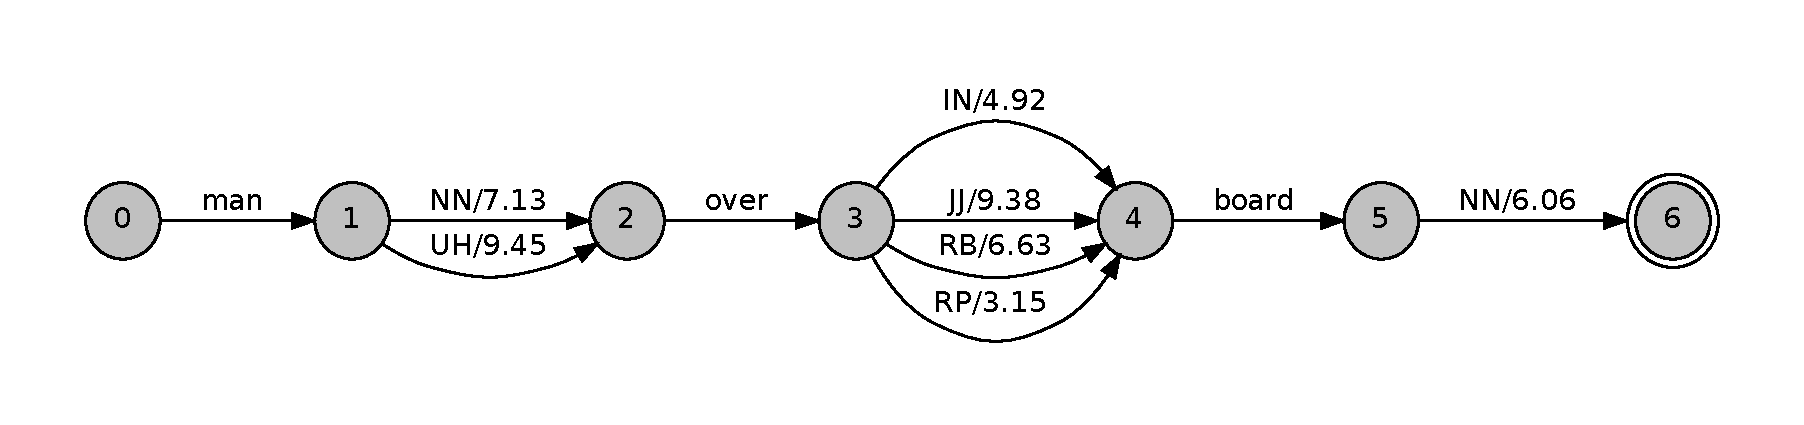
\includegraphics[scale=0.49]{sentence_model}
\caption{An example of a sentence model. The weights on the arcs are
  negative logarithms of emission probabilities. Only a subset of the
  possible labels are shown in the picture.}\label{fig:sentence-model}
\end{figure}

\paragraph{Transition Model} As stated above, Publications \ref{pub:1}
and \ref{pub:2} represent labeled sentences as a sequence of pairs
where each pair consists of a word form and a label. The transitions
model assigns weight to such sequences. I will explain the
construction of the transition model in three phases:
\begin{enumerate}
\item How to construct a model which assigns weight $-\log(p(y_{n+1}\cond
y_{1}, ..., y_{n}))$ to plain label n-grams $y_1, ..., y_{n+1}$.
\item How to extend the model to assign weight to an n-gram of word form label pairs.
\item How to score an entire labeled sentence.
\end{enumerate}
The construction presented below will result in a number of
deterministic finite-state machines whose combined effect (the
intersection of the machines) corresponds to the n-gram model in a
standard HMM.

\paragraph{Scoring one label n-gram} The transition distributions $p(y_i\cond
y_{i - 1}, ..., y_{i - n})$ in an $n$th order HMM encode the likelihood of
label sequences. I will first consider the problem of constructing a
machine which represents transition weights for isolated label
n-grams. 

To emulate transitions weights in an HMM using finite-state calculus,
we can first compile a machine $T$ which accepts any sequence of $n+1$
labels $y_{1}, ..., y_{n+1}$. The weight assigned by the machine to
one of these paths can be estimated from a training corpus for all
sequences that occur in the corpus. Some form of smoothing is required
to score label n-grams missing from the training corpus. In
Publication \ref{pub:2}, a very simple form of smoothing is used. Each
n-gram, not occurring in the training corpus, receives an identical
penalty weight $-\log(1/(N+1))$, where $N$ is the size of the training
corpus. %Additionally, Publication \ref{pub:2} uses interpolation of
%probability estimates of n-grams of different orders. 
%More
%sophisticated smoothing schemes could also be applied at the cost of
%larger model sizes.

%[WRITE ABOUT DETERMINIZATION AND MINIMIZATION]

The machine $T$ will be quite large. If it is deterministic and has one path corresponding to
each label n-gram $y_1, ..., y_{n+1}$, where $y_i \in \mathcal{Y}$, each
non-terminal state in the machine will have $\mathcal{Y}$
transitions. Because $T$ encodes the weight $p(y_{n+1}\cond y_{1},
..., y_{n})$ for each label n-gram, it will have a large amount of
states when many label n-grams occur in the training corpus. It is
difficult to present a formal analysis of the size of $T$ as a
function of the number of distinct label n-grams in the corpus. An
example can, however, illustrate the number of states that are
typically required.

For the FinnTreeBank corpus, 8801 non-terminal states are required to
represent $T$ for $n=2$. As the corpus has $1399$ distinct
morphological labels, this translates to approximately 12 million
transitions. When using add one smoothing for label n-grams missing in
the training corpus, most paths will have the same weight. This fact allows for an optimization which substantially reduces the size of $T$.

In order to, reduce the size of the model, so called {\it failure
  transitions} can be used \citep{Knuth1977,Mohri1997}.\footnote{The failure
  transitions used by \cite{Mohri1997} differ from the ones used in
  this thesis because they do not consume input.} A failure transition
in a state $q$, will match any symbol which does not have another
outgoing transition in $q$. The failure transitions will go to sink
states, which encode the penalty weight for unseen label n-grams. When
failure transitions are used to encode label n-grams that are missing
from the training corpus, most states will only have a few outgoing
transitions.  Figure \ref{fig:fail_t} illustrates a bigram model with
failure transitions.

\begin{figure}
\begin{center}
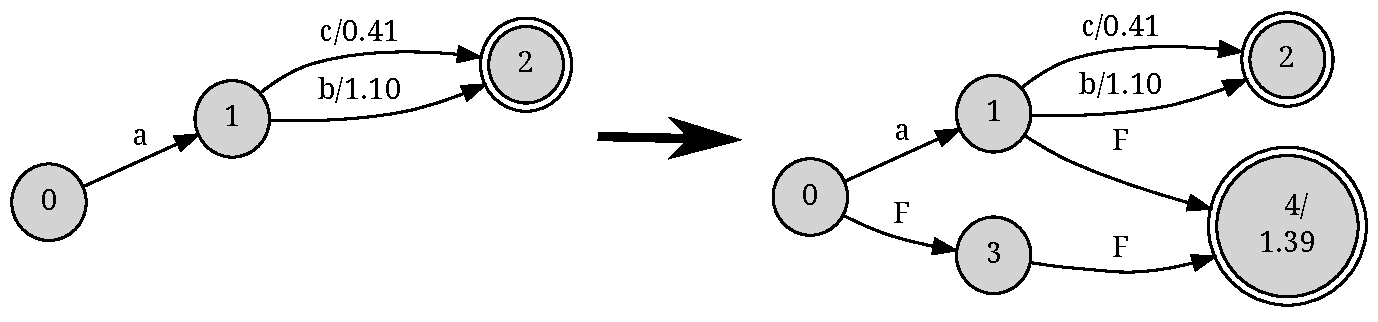
\includegraphics[scale=0.5]{fail_t}
\caption{Failure transitions (with symbol F) are added to a bigram model. With failure transitions, the model will accept previously missing n-grams, such as aa and bb with penalty weight 1.39.}\label{fig:fail_t}
\end{center}
\end{figure}

I will now outline the procedure to compute a machine with failure
transitions in the general case. We first need an auxiliary
definition. For a state $q \in Q_T$, let $n(q)$ be the length of the
shortest symbol string required to reach state $q$ from the initial
state $q_0$.  Now, given a machine $T$ that recognizes every label
n-gram {\it occurring in the training corpus}, a corresponding machine $T_f$
with failure transitions can be computed.

\begin{enumerate}
\item $n+1$ new sink states are added: $Q_{T_f} = Q_T \cup \{s_1, ...,
  s_{n+1}\}$. The state $s_{n+1}$ is final and its final weight is the
  penalty weight for unseen n-grams.
\item A failure symbol is added: $\Sigma_{T_f} = \Sigma_T \cup \{f\}$, where $f \notin \Sigma_T$.
\item Transitions are copied from $T$: $\tau_{T_f}(q,a) = \tau_T(q,a)$ for all $q \in Q_T$ and $a \in \Sigma_T$. 
\item $\tau_{T_f}(s_1,f) = \{(s_{i+1}, \mathbb{1})\}$ for $i <= n$.
\item Failure transitions are added: $\tau_{T_f}(q, f) = \{(s_{n(q)+1}, \mathbb{1})\}$, for all $q \in Q_T$.
%\item ${\rm f}(s_{n+1}) = w_p$, where $w_p$ is a penalty weight.
\end{enumerate}

\paragraph{Adding word forms} The current transition model scores
label n-grams. However, because we represent labeled sentences as
sequences of word form label pairs, we need to include word forms in
the model. This can be accomplished by adding a number of new states
and failure transitions to the model. When implementing a standard HMM
tagger, the added failure transitions will simply skip word
forms. Figure \ref{fig:fail_t_wf} demonstrates the construction for
the transition model in Figure \ref{fig:fail_t}.

\begin{figure}[!htb]
\begin{center}
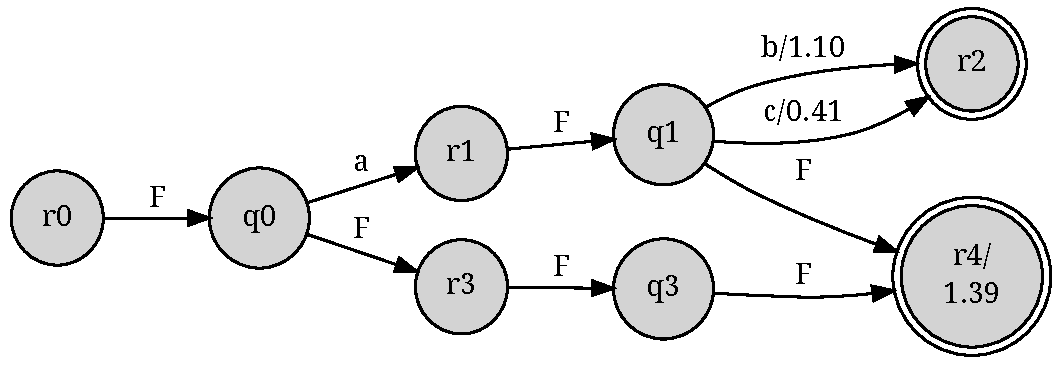
\includegraphics[scale=0.5]{fail_t_wf}
\caption{The transition model in Figure \ref{fig:fail_t} is augmented
  with failure transitions and states in order to be able to handle
  word forms.}\label{fig:fail_t_wf}
\end{center}
\end{figure}

We construct a new machine $T_w$ which accepts n-grams of word
form label pairs. Let $Q_{T_f} = \{q_0, ..., q_k\}$, then $Q_{T_w} =
Q_{T_f} \cup {r_0, ..., r_k}$, where $r_i \notin Q_{T_f}$. Let $r_0$
be the start state of $Q_{T_f}$ and let $F_{T_f} = F_{T_w}$. The
transitions function $\tau_{T_w}$ is defined in the following way.

\begin{enumerate}
\item $\tau_{T_w}(r_i,f) = \{(q_i,\mathbb{1})\}$.
\item $\tau_{T_w}(q_i,x) = \{(r_j,w)\}$ for all $x \in \Sigma_{T_w}$, if $\tau_{T_f}(q_i,x) = \{(q_j,w)\}$.
\end{enumerate}

Consider two states $q_1,q_2 \in Q_M$, in a machine $M$ with failure
transitions. Failure transitions in $q_1$ and $q_2$ may match a
different set of symbols. For example, If $q_1$ has a transition with
symbol $a \in \Sigma_M$ and $q_2$ does not, then $a$ will match the
failure transition in $q_2$ but it will not match the failure
transition in $q_1$. This is a problem when the determinization
algorithm is applied to $M$ because determinization joins states.
State joining may change the language accepted by $M$ and the
weights assigned to strings. 

It is highly desirable that the transition model of the finite-state
implementation of an HMM tagger is deterministic because of reduced
tagging time. However, as noted above, we cannot use standard
determinization with machines which have failure
transitions. Therefore, the construction presented below will produce
deterministic machines without resorting to determinization.

\paragraph{Scoring a sentence} We will now see how the transition
model for scoring an isolated label n-gram can be extended for scoring
an entire sentence. Given the machine $T_w$ which scores one n-gram,
we can form the Kleene closure of $T_w$. Since $M_n$ is an acyclic
machine accepting strings of equal length (that is $2n$: $n$ word
forms and $n$ labels), we can easily compute a deterministic Kleene
closure $T_{w}^*$ of $T_w$ by re-directing transitions going to final
states into the initial state\footnote{It can easily be seen that this
  construction fails if the machine accepts strings of unequal
  lengths.}
\begin{enumerate}
\item $\Sigma_{T_w^*} = \Sigma_{T_s}$. 
\item $Q_{T_w^*} = Q_{T_w} - F_{T_w}$.
\item $F_{T_w^*} = \{q_0\}$ and $f(q_0) = \mathbb{0}$.
\item $\tau_{T_w^*}(a,q) = \{(q', w)\}$, if $\tau_{T_w}(a,q) = \{(q',
  w)\}$ and $q'\notin F_{T_w}$.
\item If $\tau_{T_w}(a,q) = \{(q', w)\}$ and $q' \in F_{T_w}$, then
  $\tau_{T_w^*}(a,q) = \{(q_0, w + f(q'))\}$.
\end{enumerate}

The machine $T_{w}^*$ will score entire labeled sentences, however, it
only scores some of the trigrams in the sentence, namely, the ones
starting at positions divisible by $n+1$. Fortunately we can form $n +
1$ machines $T_0$ ... $T_n$ which will score all remaining
n-grams. Let $T_0 = T_{w}^*$ and let $T_{i+1} = F.F.T_i$. Intuitively
each $T_i$ will skip $i$ word form label pairs.

The final scoring of all possible labeled sentences, corresponding to
an input sentence $x$, is accomplished by intersecting the sentence
model $X$ and each of the $T_i$ using an intersection algorithm which
handles failure symbols correctly. In Publications \ref{pub:1} and
\ref{pub:2} a parallel intersection algorithm \citep{Silfverberg2009},
however, this is not actually required. The intersections can be
performed sequentially.

\paragraph{Smoothing} As observed in Chapter \ref{chapter:hmm}, a
second order model usually gives the best results in morphological
tagging. However, a pure second order model suffers from data sparsity
which degrades it performance. This can be avoided using smoothing. In
Publications \ref{pub:1} and \ref{pub:2}, smoothing is accomplished by
using first and zeroth order transition models in addition to the
second order transition model. To get the combined effect of all
models, each of them is intersected with the sentence model.

Usually, for example in \cite{Brants2000}, the transition
probabilities $p(y_i|y_{i-1}, y_{i-2})$ are a linear interpolation of
the probability estimates $\hat{p}$ for different orders as shown in
equation \ref{eq:ip}. \cite{Brants2000} sets the values for $\alpha_i$
using deleted interpolation and cross validation. When $\sum_i
\alpha_i = 1$, it is easily seen that Equation \ref{eq:ip} defines a
probability distribution over $y_i$.

\begin{equation}
p(y_i|y_{i-1}, y_{i-2}) = \alpha_2\hat{p}(y_i|y_{i-1},y_{i-2}) + \alpha_1\hat{p}(y_i|y_{i-1}) + \alpha_0\hat{p}(y_i)\label{eq:ip}
\end{equation}

Linear interpolation is not possible when using the finite-state
implementation presented in this chapter because intersection of
weighted machines corresponds to multiplying probability estimates,
not to adding them. Therefore, Publications \ref{pub:1} and
\ref{pub:2} define the score $s(y_i|y_{i-1}, y_{i-2})$ of a labeled
sentence as the weighted product given in Equation
\ref{eq:ip-fsm}. Inference corresponds to finding the label sequence
which maximizes the score. The optimal values for the exponents
$\alpha_i$ in Equation \ref{eq:ip-fsm} are found by optimizing the
tagging accuracy on held out data using grid search.

\begin{equation}
s(y_i|y_{i-1}, y_{i-2}) = \hat{p}(y_i|y_{i-1},y_{i-2})^{\alpha_2} \hat{p}(y_i|y_{i-1})^{\alpha_1}\hat{p}(y_i)^{\alpha_0}\label{eq:ip-fsm}
\end{equation}

The weighted product $s(y_i|y_{i-1}, y_{i-2})$ given by
\ref{eq:ip-fsm} does not necessarily define a probability distribution
over $y_i$. It can, however, easily be normalized to give one. When the
score is normalized, it can be seen as a special case of the family of
distributions defined by Equation \ref{eq:ip-general}. Here the
parameter values $r_2(y_i|y_{i-1},y_{i-2})$, $r_1(y_i|y_{i-1})$,
$r_0(y_i)$ can be arbitrary positive real numbers. Each assignment of
the parameter values defines a probability distribution over $y_i$.

\begin{equation}
p(y_i|y_{i-1}, y_{i-2}) = \frac{r_2(y_i|y_{i-1},y_{i-2})r_1(y_i|y_{i-1})r_0(y_i)}{\sum_{y\in\mathcal{Y}} r_2(y|y_{i-1},y_{i-2})r_1(y|y_{i-1})sr0(y)}\label{eq:ip-general}
\end{equation}

The interpretation of the weighted product in Equation \ref{eq:ip-fsm}
given by Equation \ref{eq:ip-general} reveals a problem. There is no
guarantee that the parameter values $r(y_i|y_{i-1},y_{i-2}) =
\hat{p}(y_i|y_{i-1},y_{i-2})^{\alpha_2}$, $r_1(y_i|y_{i-1}) =
\hat{p}(y_i|y_{i-1})$ and $r_0(y_i) = \hat{p}(y_i)^{\alpha_0}$ result
in a model which fits the training data maximally well in the sense
that is discussed in Chapter \ref{chap:ml}. This may have contributed
to the inferior tagging accuracy of the system when compared to
\cite{Brants2000} which is seen in the experiments in Publication
\ref{pub:2}. This problem lead the
author to consider conditional random fields presented in Chapter
\ref{chapter:crf}, which naturally support a product formulation.

\section{Beyond the Standard HMM}\label{sec:enriched}

The real strength of the system presented in this chapter lies in its
capability of easily incorporating information not usually present in
a generative HMM tagger. \cite{Halacsy2007} show that enriching the
emission model of an HMM tagger by including label context can improve
tagging results. Instead of the usual emission model $p(x_t\cond y_t)$
which conditions each word on its morphological label,
\cite{Halacsy2007} instead use a model $p(x_t\cond y_{t-1},y_t)$,
where the emission is conditioned on preceding label context. As
stated in Chapter \ref{chapter:hmm}, this is in fact not an extension
to the standard second order HMM. Instead, it is the faithful
implementation of the second order HMM model. The definition
$p(x_t\cond y_t)$, used by for example \cite{Brants2000}, is incorrect
in a second order HMM. It is probably used because of data
sparsity. Nevertheless, \cite{Halacsy2007} show that the correct
formulation can result in improved tagging accuracy.

\paragraph{Richer local structure} The model presented by
\cite{Halacsy2007} can easily be implemented as a finite-state machine
by a slight modification to the compilation of the sentence model as
described in Publication \ref{pub:1} and it can be extended to model
$p(x_t\cond y_{t-1}, y_t, y_{y+1})$. Moreover, it is possible to
condition transitions on word forms as shown in Publication
\ref{pub:1}. Both of these modifications are shown to give
statistically significant improvements over the standard baseline
model. The problem with including such information in the emission and
transition models is that it violates the conditional independence
assumptions in the generative HMM model. This is yet another reason to
consider alternative models such as the conditional random field or
averaged perceptron.

\paragraph{Global Constraints} In addition to local changes to the
emission and transition models, it would also be possible to include
global probabilistic constraints to the model. These are constraints
that apply on the entire input sentence. A simple example of such a
constraint is the existence or frequency of finite verb forms in the
sentence. Another family of interesting global constraints is given by
syntactic and semantic valency of words \citep{Baker1998}. Such
information could be represented as a weighted finite-state
machine. Similarly to the enriched locally emission and transition
models, global constraints also violate the independence assumption of
the generative HMM model.

\section{Summary of Publications \ref{pub:1}, \ref{pub:2} and \ref{pub:3}}

Publication \ref{pub:1} presents the finite-state implementation of
HMMs introduced in this Chapter and Publication \ref{pub:2} presents
experiments using the model on the Penn Treebank and a Finnish data
set. The taggers presented in Publications \ref{pub:2} are used in
Publication \ref{pub:3} to implement a language model for a
context-sensitive finite-state spelling corrector.

\paragraph{Publication \ref{pub:1}} The main contribution of this
publication is to present the finite-state implementation of HMMs. The
publication presents experiments on morphological tagging of Finnish,
English and Swedish but the experiments presented in the publication
are nearly void of value because they were conducted on machine
labeled data and the amount of training data was unrealistic (1
million sentences for each language). Both factors contribute to
extremely good, and quite unrealistic, tagging accuracy for all
languages on test data. Still, the extreme size of the training set
does demonstrate that the method can use large amounts of training
data.

For Finnish, experiments on machine labeled data were the only option
because, at the time, there was no freely available hand-labeled
morphologically tagged corpus available. For Swedish and English,
established data sets should have been used.

The formulation of the probabilistic model in Publication \ref{pub:1}
differs from the formulation in this Chapter in two respects. Instead
of the usual transitions probabilities $p(y_{t}\cond y_{t-n}, ...,
y_{t-1})$, Publication \ref{pub:1} uses the joint probability
$p(y_{t-n}, ..., y_t)$. The model can therefore not be seen as an
actual HMM. Additionally, the publication uses lexicalized transition
probabilities. The final probability is thus $p(l_{t-n}, y_{t-n}, ...,
l_t, y_t)$, where the $l$ refer to lemmas. This is possible because of
the extremely large training set.

Although the experiments in Publication \ref{pub:1} are flawed, the
paper is included in the thesis because it describes the finite-state
implementation for HMM taggers and can be seen as a natural starting
point for Publications \ref{pub:2} and \ref{pub:3}.

\paragraph{Publication \ref{pub:2}} The main contribution of this
publication is to present experiments on a standard data set for POS
tagging of English, the Penn Treebank 2. However, because of
insufficient knowledge at the time, the experiments were performed on
a non-standard version of Penn Treebank 2. Publication \ref{pub:1}
uses the data splits introduced by \cite{Collins2002} but the data
from the {\tt tagged} sub-directory in the Penn Treebank 2
distribution. As \cite{Toutanova2003} explain, it is conventional to
extract the POS tagged sentences from the parse trees in the {\tt
  parsed} sub-directory in the distribution. Unfortunately, this makes
the reported accuracies approximately 0.3 \%-points higher than they
would be if the experiments were performed on the correct data
set. For Finnish, experiments were performed on machine labeled data by
necessity, similarly as in the case of Publication \ref{pub:1}.

Publication \ref{pub:2} presents models for Finnish and English which
use enriched emission models described in Section \ref{sec:enriched},
which are inspired by the HunPos system \citep{Halacsy2007}. The
taggers are evaluated against a standard HMM baseline. The results are
also compared against tagging accuracies reported in \cite{Brants2000}
and \cite{Halacsy2007}. Because of the unfortunate mix-up with the
Penn Treebank data set, the results for English are not comparable
between the different tagging systems. However, Publication
\ref{pub:2} does show that the enriched emission models yield clear
improvements over baseline. Moreover, the final system outperforms
HunPos by 0.4\%-points on the Finnish data set. Because the data set
is machine labeled, this result may of course not be convincing.

\paragraph{Publication \ref{pub:3}} This publication applies the
taggers presented in Publications \ref{pub:1} and \ref{pub:2} to the
task of context-sensitive spelling correction. Many spelling
correction systems determine the best spelling correction for a
misspelled word based solely on the misspelled word form
itself. Typically, correction candidates that have a small edit
distance to the misspelled word form are ranked higher than more
remote candidates. Context-sensitive spelling correction systems
additionally utilize surrounding words to rank correction candidates.

For English, plain word context can improve the accuracy of spelling
correction \citep{Brill2000}. For example ``cat'' is much more likely
in the context ``the _ miaowed'' than ``car'' is. As Publication
\ref{pub:2} shows, word context does improve results for Finnish as
well. However, Publication \ref{pub:3} also shows that a morphological
tagger can yield greater improvements in accuracy for both English and
Finnish when using comparable amounts of training data for the tagger
and word context model. Of course, the word context model can be
trained on unlabeled data. Therefore, there is in principle no
obstacle to using arbitrarily much training data.

The system presented in Publication \ref{pub:3} first generates a set
of correction candidates for the misspelled word using a finite-state
spelling correction system based on edit distance. It then uses a
generative morphological tagger for selecting the best candidate. The
misspelled form is replaced with each correction candidate $c_1$, ...,
$c_n$ in turn producing $n$ sentences $x_1$, ..., $x_n$. The sentences
are then tagged which results in $n$ tag sequences $y_1$, ...,
$y_n$. The candidates $c_i$ are finally ranked according to the joint
probability of the sentence and label sequence
$p(y_i,x_i)$.\footnote{In fact only a sub-sequence of the sentence is
  tagged as an optimization, however, the basic idea is the same.}

The spelling correction system using the morphological tagger probably
yields better results, especially for English, because it is less
susceptible to data sparsity than the word context model. As noted
above, the amount of training data for the word context model could,
however, be increased. This is likely to gradually improve
accuracy. At the same time it, however, increases the size of the
model. The spelling correction system that uses the morphological
tagger can be more compact and thus more practicable while delivering
comparable accuracy.
